 \documentclass[11pt]{article}
\usepackage[a4paper, hmargin={2.8cm, 2.8cm}, vmargin={2.5cm, 2.5cm}]{geometry}
\usepackage{eso-pic} % \AddToShipoutPicture
\usepackage{graphicx} % \includegraphics
\usepackage{framed}
\usepackage[utf8]{inputenc}
\usepackage{hyperref}
\usepackage{amsmath} % flere matematikkommandoer
\usepackage{amssymb} % flere matematikkommandoer
\usepackage{amsfonts}              % for blackboard bold, etc
\usepackage{amsthm}                % better theorem environments
\usepackage[utf8]{inputenc} % æøå
\usepackage[T1]{fontenc} % mere æøå
\usepackage{verbatim} % så man kan skrive ren tekst
\usepackage[all]{xy} % den sidste (avancerede) formel i dokumentet
\usepackage{graphicx}              % to include figures
\usepackage{caption}
\usepackage{bm}
\usepackage{fancyhdr}
\usepackage{mathtools}
\usepackage{listings}
\usepackage{enumitem}
\usepackage{breqn}
\usepackage{tikz}
\usepackage{mdframed}
\usetikzlibrary{arrows,automata,fit,positioning, shapes, arrows.meta,chains,matrix,decorations.pathreplacing, calc}
\newcommand\doubleplus{+\kern-1.3ex+\kern0.8ex}
\newcommand\lett{\phantom{-}\:\:\mathbf{let}\:\:}
\newcommand\inn{\:\:\mathbf{in}\:\:}
%% Change `ku-farve` to `nat-farve` to use SCIENCE's old colors or
%% `natbio-farve` to use SCIENCE's new colors and logo.
\def \ColourPDF {include/nat-farve}

%% Change `ku-en` to `nat-en` to use the `Faculty of Science` header
\def \TitlePDF   {include/nat-en}  % University of Copenhagen

\title{
  \vspace{3cm}
  \Huge{Implementing Map-Scan Fusion in the Futhark Compiler} \\
  \Large{Bachelor project}
}

\author{
  \Large{Brian Spiegelhauer}
  \\ \texttt{brianspieg@gmail.com} \\ \\
   \Large{William Jack Lysgaard Sprent}
  \\ \texttt{bsprent@gmail.com} \\
}

\date{
    \today
}

\begin{document}
\lstset{language=C, frame=single, numbers=left, breaklines=true}
\mdfdefinestyle{alignbox}{leftmargin=100pt,
rightmargin=100pt,%
innerleftmargin=10pt,
innerrightmargin=10pt,
innertopmargin=0.1pt,
innerbottommargin=0.1cm,
skipbelow=10pt}

\AddToShipoutPicture*{\put(0,0){\includegraphics*[viewport=0 0 700 600]{\ColourPDF}}}
\AddToShipoutPicture*{\put(0,602){\includegraphics*[viewport=0 600 700 1600]{\ColourPDF}}}

\AddToShipoutPicture*{\put(0,0){\includegraphics*{\TitlePDF}}}

\clearpage\maketitle
\thispagestyle{empty}

\newpage

\tableofcontents

\newpage

\section{Abstract}
\section{Introduction}
\textit{NOTE: the contents of this section is lifted from our synopsis and is probably placeholder}\\
The Futhark language is a functional programming with which the main idea is to allow for the expression of sufficiently complex programs while keeping complexity to a level where programs can be aggressively optimised and have their parallelism exploited \cite{futharkdoc}.

The Futhark compiler already supports a range of fusion optimisations \cite{T2Fusion}, but does not currently support fusion between \texttt{Map} and \texttt{Scan} statements.

For our project we will explore the possibility of implementing Map-Scan fusion into the Futhark compiler, and will examine the performance benefits (if any) of performing such optimisations.

\subsection{Motivation}
Fusion has the ``[..] potential to optimize both the memory hierarchy time overhead and, sometimes asymptotically, the space requirement" \cite{T2Fusion}. Hence the main motivation for adding Map-Scan fusion capabilities to the optimiser of the Futhark compiler, is the potential for enabling performance increases for some Futhark programs.

\subsection{Tasks}
The project can be divided into three main tasks:
\begin{enumerate}
    \item Gain an understanding of logical reasoning behind fusion optimisations on Second Order Array Combinators.
    \item Read and understand the relevant parts of the Futhark compiler required to make the necessary changes in the compiler.
    \item Modify all modules of the Futhark compiler necessary to implement the Map-Scan fusion itself.
\end{enumerate}
At first sight, these tasks look fairly straight forward. However, we expect that the main difficulties of this project lie within unforeseen roadblocks we will run into when modifying the codebase.

\section{Background Information}
%Describe some relevant background info for how SOACs are parallelly computed - relevant %to why Scanomap is smart. IMPORTANT: WHY MEMORY MANAGEMENT IS VERY IMPORTANT ON GPU\\

There are problems/calculations that gets to a size where normal sequential programming involving consecutive execution of processes, will reach a computation time unsatisfying for the intended users. In some cases these calculations can be done much faster with parallel programming. Parallel programming is where many calculations are carried out simultaneously, with the idea of dividing a problem into smaller sub problems solved at the same time. Parallel and sequential programming are not mutually exclusive, in the sense that if you use parallel programming, you cant use sequential programming, in many cases they are used together. Parallel programming can be done on the CPU with its multiple cores, but when possible and advantages it is much better to harness the thousands of cores in the GPU - graphics processing units. The GPU is no longer only used to do graphical calculations, but also General-purpose computing, GPGPU (General-purpose computing on graphics processing units). \\

To do GPGPU, Hyperfit a joint research center addressing the simultaneous challenges of high transparency, high computational performance and high productivity in finance, employing an integrated approach of financial mathematics, domain specific languages, parallel functional programming, and high-performance systems \cite{Hyperfit} created Futhark. 


\subsection{Futhark}
As described in Troels Henriksens master thesis \cite[The $\mathcal{L}_0$ language, p. 8]{MasterTroels} the language $\mathcal{L}_0$ later renamed Futhark is in a sense "sufficient", in that it is Turing-complete, and can express imperative style loops with do-loops. However Futhark is ment to use second-order array combinations (SOACs) to do bulk operations on arrays instead of using the do-loops. In this sections the reasoning behind using SOACs will be explained by showing the difference in their computation when done sequentially vs. parallelly.
%Chunking
\subsection{SOACs}
Both \texttt{map} and \texttt{scan} are defined as SOACs -- or Second Order Array Combinators. Hence they have no free variables, take first-order functions as arguments, and output first-order
 functions whose domains are arrays of the domain of the input. Furthermore, in Futhark, these array inputs and outputs are tuples of arrays, and not arrays of tuples.
While Futhark SOACs are semantically identical to their namesake higher-order functions found in other functional languages, working with SOACs allows for some assumptions to be made
 which turn out to be useful in regards to both parallisation and optimisation. In particular each SOAC can be considered as representing a specific shape of an imperative do-loop, which
 is used in Futhark to expedite the loop-fusion process. \cite[chap. 7]{MasterTroels}

Futhark SOACs work with tuples of arrays in favour of arrays of tuples. This means that when talking about input or output array to a SOAC, we are talking about an arbitrary amount of arrays with
 the same length. For example, $b = \mathtt{map} \: f \: a$ is in fact short hand for $(b0, b1,..., bn) = \mathtt{map} \: f \: (a0, a1, ..., am)$ where $ai$ and $bj$ are each arrays, and each of the arrays
 in a tuple have the same amount of
 elements.
% Definition of SOACs
% Why are they useful wrt. parallelisation
% Soacs with tuples in Futhark
\subsubsection{Map}
The $\texttt{map} \: f \: a$ function, has the very simple definition of taking a function $f \: : \: \alpha \to \beta$ and returning a function $\mathtt{map} \:f \: : \: [\alpha] \to [\beta]$  which
 applies $f$ to every element of an input array, $a$.  This gives us the type signature of \texttt{map},
$$\mathtt{map} \: f \: a \: :  \: (\alpha \to \beta) \to [\alpha] \to [\beta]\mathnormal{.}$$
And the semantic definition of \texttt{map},
$$\mathtt{map} \: f \: a \: =  \: [f(a_0), f(a_1), ..., f(a_{n-1})]\mathnormal{.}$$
Having no free variables, means that each result $f(a_i)$ \textit{only} depends on the corresponding element $a_i$. This makes \texttt{map}s fantastic for parallelisation as once the
 degree of parallism reaches the size of $a$, $\mathtt{map} \: f \: a$ can be potentially be computed in a single parrallel step, or $c$ steps for a chunk size of $c$.

 \begin{figure}[h!]
   \centering
   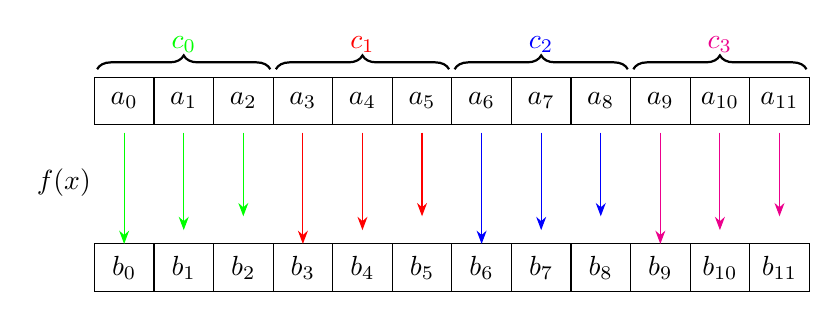
\begin{tikzpicture}[ node distance=0pt, start chain = A going
     right, start chain = C going right, arrow/.style =
     {draw=#1,-{Stealth[]}, shorten >=1mm, shorten
       <=1mm}, % styles of arrows
     arrow/.default = black, X/.style = {rectangle,
       draw,% styles of nodes in string (chain)
       minimum width=5ex, minimum height=4ex, outer sep=0pt, on
       chain}, B/.style = {decorate, decoration={brace, amplitude=5pt,
         pre=moveto,pre length=1pt,post=moveto,post length=1pt,
         raise=1mm, #1}, % for mirroring of brace, if necessary
       thick}, B/.default = mirror, % by default braces are mirrored
     ]
     \foreach \i in {0,...,11}% <-- content of nodes
     \node[X, on chain = A] {$a_\i$};

     \node [X, on chain = C, below = 10ex of A-1] {$b_0$}; \foreach \i
     in {1,...,11}% <-- content of nodes
     \node[X, on chain = C] {$b_\i$};

     ; \draw[B=] (A-1.north west) -- coordinate[above=3mm] (a1)
     (A-3.north east) node [green, midway, above, yshift = 5pt] (a)
     {$c_0$}; \draw[B=] (A-4.north west) -- coordinate[above=3mm] (a2)
     (A-6.north east) node [red, midway, above, yshift = 5pt] {$c_1$};
     \draw[B=] (A-7.north west) -- coordinate[above=3mm] (a3)
     (A-9.north east) node [blue, midway, above, yshift = 5pt]
     {$c_2$}; \draw[B=] (A-10.north west) -- coordinate[above=3mm]
     (a4) (A-12.north east) node [magenta, midway, above, yshift = 5pt]
     {$c_3$};


     \foreach \c [count=\i] in {green, red, blue, magenta} { \foreach
       \j in {1,...,3} { \pgfmathtruncatemacro{\is}{\i - 1}%
         \pgfmathtruncatemacro{\jn}{\is * 3 + \j}%
         \pgfmathtruncatemacro{\jl}{(\j - 1) * 5}%
         \draw[arrow,\c , shorten >= \jl pt] (A-\jn.south) to
         (C-\jn.north) node (AR-\jn) {}; } }

     \node [above left= 10pt and 5pt of AR-1] {$f(x)$};

   \end{tikzpicture}
   
   \caption{Parallel computation of map with chunking. Each colour represents a seperate thread.}
   \label{fig:compmap1}
 \end{figure}

Figure \ref{fig:compmap1} displays how map can be computed in chunks. Each thread is responsible for sequentially computing
 $\mathtt{map} \: f \: c_i$ across a single chunk. With no depedencies in the way, this can happen in parallel such that the
 12 element list is \texttt{map}ped with just 3 sequential applications of $f$.
% INSERT COOL FIGURE OF MAP BEING COMPUTED 
% How do we compute it parallely
% Timecomplexity?

\subsubsection{Scan}
% what is a scan
$\texttt{scan} \: \odot \: e \: a$ takes a binary, associative function $\odot \: : \: \alpha \to \alpha \to \alpha$ and returns a function
 $\mathtt{scan} \:\odot \: : \: \alpha \to [\alpha] \to [\alpha]$ which
 computes the $\odot$ prefixes of an input array $a$ starting with a neutral element, $e$. Overall, \texttt{scan} has the type signature,
$$\mathtt{scan} \: \odot \: e \: a \: : \:(\alpha \to \alpha \to \alpha) \to \alpha \to [\alpha] \to [\alpha]\mathnormal{.}$$
Computing \texttt{scan} with the function $\odot$, the array $a$, and neutral element $e$ gives us,
$$\mathtt{scan} \: \odot \: e \: a \: = [e \odot a_0, e \odot a_0 \odot a_1, ..., e \odot a_0 \odot ... \odot a_{n-1}]\mathnormal{.}$$
% How do we compute it parallely
However, computing such a \texttt{scan} is not as simple as with a \texttt{map} as each prefix $a_0 \odot ... \odot a_i$ obviously depends on the previous prefix $a_0 \odot ... \odot a_{i-1}$. Hence, 
the associativity of $\odot$ is vital as it means that this dependency does not force computation order, and partial results can be computed independently and combined.
% How scan is computed in Futhark with fancy diagram 

% Timecomplexity?
\begin{figure}[h!]
  \centering
  \begin{tikzpicture}[ node distance=0pt,
    start chain = A going right,
    start chain = C going right,
    start chain = D going right, 
    start chain = E going right,
    start chain = G going right,
    arrow/.style = {draw=#1,-{Stealth[]},shorten >=1mm, shorten <=1mm}, % styles of arrows
    arrow/.default = black, X/.style = {rectangle, draw,% styles of nodes in string (chain)
      minimum width=7ex, minimum height=4ex, outer sep=0pt, on chain},
    B/.style = {decorate, decoration={brace, amplitude=5pt,
        pre=moveto,pre length=1pt,post=moveto,post length=1pt,
        raise=1mm, #1}, % for mirroring of brace, if necessary
      thick},
    B/.default = mirror, % by default braces are mirrored
    ]
    \foreach \i in {0,...,11}% <-- content of nodes
    \node[X, on chain = A] {$a_\i$};

    \node [X, on chain = C, below = 10ex of A-1] {$a_0$};
    \node [X, on chain = C] {$a_{0-1}$};
    \node [X, on chain = C] {$a_{0-2}$};
    \foreach \i in {3, 6, 9} { 
      \node[X, on chain = C] {$a_\i$};
      \foreach \j in {1,...,2} { 
        \pgfmathtruncatemacro{\ij}{\i + \j}%%
        \node[X, on chain = C] {$a_{\i-\ij}$}; 
      }
    }

    \node [X, on chain = D, below = 10ex of C-1] {$a_0$};
    \node [X, on chain = D] {$a_{0-1}$};
    \node [X, on chain = D] {$a_{0-2}$};
    \node [X, on chain = D] {$a_{3}$};
    \node [X, on chain = D] {$a_{3-4}$};
    \node [X, on chain = D] {$a_{0-5}$};
    \node [X, on chain = D] {$a_{6}$};
    \node [X, on chain = D] {$a_{6-7}$};
    \node [X, on chain = D] {$a_{3-8}$};
    \node [X, on chain = D] {$a_{9}$};
    \node [X, on chain = D] {$a_{9-10}$};
    \node [X, on chain = D] {$a_{6-11}$};

    \node [X, on chain = E, below = 10ex of D-1] {$a_0$};
    \node [X, on chain = E] {$a_{0-1}$};
    \node [X, on chain = E] {$a_{0-2}$};
    \node [X, on chain = E] {$a_{3}$};
    \node [X, on chain = E] {$a_{3-4}$};
    \node [X, on chain = E] {$a_{0-5}$};
    \node [X, on chain = E] {$a_{6}$};
    \node [X, on chain = E] {$a_{6-7}$};
    \node [X, on chain = E] {$a_{0-8}$};
    \node [X, on chain = E] {$a_{9}$};
    \node [X, on chain = E] {$a_{9-10}$};
    \node [X, on chain = E] {$a_{0-11}$};




    \node [X, on chain = G, below = 10ex of E-1] {$a_0$};
    \node [X, on chain = G] {$a_{0-1}$};
    \node [X, on chain = G] {$a_{0-2}$};

    \foreach \i in {3,...,11} {
      \node[X, on chain = G] {$a_{0-\i}$};
    }


    \draw[B=] (A-1.north west) -- coordinate[above=3mm] (a1)
    (A-3.north east) node [green, midway, above, yshift = 5pt] (a)
    {$c_0$}; \draw[B=] (A-4.north west) -- coordinate[above=3mm] (a2)
    (A-6.north east) node [red, midway, above, yshift = 5pt] {$c_1$};
    \draw[B=] (A-7.north west) -- coordinate[above=3mm] (a3)
    (A-9.north east) node [blue, midway, above, yshift = 5pt] {$c_2$};
    \draw[B=] (A-10.north west) -- coordinate[above=3mm] (a4)
    (A-12.north east) node [magenta, midway, above, yshift = 5pt]
    {$c_3$};


    \foreach \c [count=\i] in {green, red, blue, magenta} {
      \foreach \j in {2,...,3} { 
        \pgfmathtruncatemacro{\is}{\i - 1}%
        \pgfmathtruncatemacro{\jn}{\is * 3 + \j}%
        \pgfmathtruncatemacro{\jl}{(\j - 2) * 5}%
        \draw[arrow,\c , shorten >= \jl pt] (A-\jn.south) to (C-\jn.north) node (AR-\jn) {};
      }
    }
    \foreach \c [count=\i] in {green, red, blue, magenta} {
      \foreach \j in {1,...,2} {
        \pgfmathtruncatemacro{\ir}{\i - 1}%
        \pgfmathtruncatemacro{\pos}{3 * \ir + \j}%
        \pgfmathtruncatemacro{\ii}{\pos +1}%
        \draw[arrow, \c] (A-\pos.south) to[out=280, in=200] (A-\ii.south) node (CR-\pos) {};
      }
    }
    \foreach \i/\c in {3/red,6/blue,9/magenta} {
      \pgfmathtruncatemacro{\iii}{\i + 3}%
      \def\this{C-\iii.south}
      \def\there{D-\iii.north}
      \coordinate (mid\i) at ($(\this) !0.6! (\there)$);
      \node at (mid\i) {$\odot$};
      \draw[arrow, \c,shorten >= 4pt] (C-\iii.south) to node[midway, black] (RED-1) {} (mid\i.north) ;
      \draw[arrow, \c,shorten >= 4pt] (C-\i.south) to[out=340 ,in=90] (mid\i.north);
      \draw[arrow, \c,shorten <= 4pt] (mid\i) to (D-\iii.north) ;

    }


    \foreach \i/\c in {3/blue,6/magenta} {
      \pgfmathtruncatemacro{\iii}{\i + 6}%
      \def\this{D-\iii.south} 
      \def\there{E-\iii.north}
      \coordinate (mid\i) at ($(\this) !0.6! (\there)$);
      \node at (mid\i) {$\odot$};
      \draw[arrow, \c,shorten >= 4pt] (D-\iii.south) to node[midway, black] (RED-1) {} (mid\i.north) ;
      \draw[arrow, \c,shorten >= 4pt] (D-\i.south) to[out=320 ,in=90, looseness=0.6] (mid\i.north);
      \draw[arrow, \c,shorten <= 4pt] (mid\i) to (E-\iii.north) ; 
    }




    \foreach \c [count=\i] in {red, blue, magenta} {
      \foreach \j in {2,...,3} {
        \pgfmathtruncatemacro{\is}{\i - 0}%
        \pgfmathtruncatemacro{\jn}{\is * 3 + \j -1}%
        \pgfmathtruncatemacro{\jl}{(\j - 2) * 3}%
        \draw[arrow,\c, shorten >= \jl pt] (E-\jn.south) to (G-\jn.north) node (GR-\jn) {};
      }
      \foreach \j in {1,...,2} { 
        \pgfmathtruncatemacro{\ir}{\i - 1}%
        \pgfmathtruncatemacro{\pos}{3 * \ir + \j + 2}%
        \pgfmathtruncatemacro{\ii}{\pos +1}%
        \draw[arrow, \c] (E-\pos.south) to[out=280, in=200] (E-\ii.south) node (GGR-\pos) {};
      }
    }
    \node [above left= 10pt and 5pt of AR-1] (other) {$\odot$};
    \node [below= 38ex of other] {$\odot$};
  \end{tikzpicture}
  
  \caption{Parallel computation of \texttt{scan} with chunking. Each colour represents a single thread, and $a_{i-j} = a_i \odot a_{i+1} \odot ... \odot a_j$.}
  \label{fig:scancomp1}
\end{figure}
With this, there are multiple ways in which \texttt{scan} can be computed in parallel with chunking, and Figure \ref{fig:scancomp1} shows a simple algorithm.
 It is a three phase process which step-wise involves,
 \begin{enumerate}
 \item First each thread sequentially computes the $\odot$-prefixes of their respective chunks. ($c$ steps)
 \item Then the final element of each chunk is recursively combined with the previous using $\odot$ with
 doubling stride for each recursion, such that each final element contains the $a_{0-j}$ prefix where $j = (c * (i+1) - 1)$ for the
 $i$th chunk. ($\log(\frac{n}{c})$ steps)
 \item Finally each thread adds the final element of the previous chunk to each element of the chunk
 which is not the tail. ($c$ steps)
 \end{enumerate}
While this algorithm is not work efficient -- it involves more than $n$ applications of $\odot$ -- it still has a running time of $O(2c + \log(n)) < O(n)$ due to parallelism.

\section{Fusion}
In this section the basic idea of loop fusion will be outlined, with a closer look at the two kinds of fusion implemented in this paper.
The loop fusion technique gives the possibility of reducing loop overhead and increase execution speed, and the potential to optimize both the memory hierarchy time overhead and space requirements. Loop fusion is as the name implies, fusing loops together. However this requires that the loops iterate the same number of times, as that could for example make one loop try to fetch data out of bounds. \\

\begin{lstlisting}[caption=Pre-fusion.]

  a[n];
  b[n];

  for (int i = 0; i < n; i++) {
    a[i] = i
  }

  for (int i = 0; i < n; i++) {
    b[i] = i
  }
\end{lstlisting}
Having two loops with the same iteration range as shown in listing 1, it gives the possibility for fusion them together as one. Both loops do the work needed within the same range, and therefore it could be done in one loop as shown in listing 2. Cases where fusion will not be possible regardless of two equal length loops, will be shown later on.

\begin{lstlisting}[caption=Post-fusion.]
  a[n];
  b[n];
  
  for (int i = 0; i < n; i++) {
    a[i] = i
    b[i] = i  
  }
\end{lstlisting}

By doing the fusion in this case, loop-overhead has been reduced in half, as now it is only necessary to keep track of one loop instruction.

\subsection{Consumer-Producer Fusion}
Consumer-Producer loop fusion is slightly more complicated. In this case the two loops are connected, as in inside the producer-loop some data is being created, that is required in the consumer-loop. I.e a producer creates some data, and a consumer uses the created data, this relationship is referred to as a producer-consumer relationship. \\
Loop fusion of a consumer-producer relationship now gives the opportunity to fuse the functions in the 2 loops into one, i.e $f(x) \circ g(x) = f(g(x))$ as the example in listing 3 and 4 shows. 

\begin{lstlisting}[caption=Producer-Consumer pre-fusion.] 
  a[n];
  b[n];
  c[n];
  	  
  for (int i = 0; i < n; i++) {
    b[i] = f(a[i]) // f(x) some function doing work  
  }
  
  for (int i = 0; i < n; i++) {
    c[i] = g(b[i]) // g(x) some function doing work
  }
\end{lstlisting}

\begin{lstlisting}[caption=Producer-Consumer post-fusion.] 
  a[n];
  c[n];
  	  
  for (int i = 0; i < n; i++) {
    c[i] = f(g(a[i])
  }
\end{lstlisting}

The result is reduced loop overhead, reducing in memory requirements as the output of the producer loop is no longer stored separately, but calculated within the fused result.

\subsection{Horizontal Fusion}
Horizontal fusion is a none producer-consumer fusion, i.e the two loops must have no connection with each other. Listing 1 and 2 therefore perfectly examples a horizontal fusion.  
\subsection{Fusion in Futhark}
Futhark is centered around SOACs for doing operations on arrays, and you do therefore not write loops to do array functions. Loop fusion for that reason is focused on SOAC fusion. The SOACs can currently be divided up as producer consumer functions as shown below:

\begin{table}[hb!]
\centering
\caption{Producers and Consumers in Futhark}
\label{my-label}
\begin{tabular}{|l|l|}
\hline
\textbf{Producers} & \textbf{Consumers} \\ \hline
Map                & Map                \\ \hline
                   & Reduce             \\ \hline
                   & Scan               \\ \hline
Filter             & Filter             \\ \hline
                   & Redomap            \\ \hline
                   & Scanomap           \\ \hline
\end{tabular}
\end{table}

\section{Map-Scan Fusion}
% Why?
In a typical situation involving \texttt{map} and \texttt{scan}, we will have the \texttt{map} producing some array, which is subsequently
 consumed by the \texttt{scan}:
\begin{align*}
  b &= \mathtt{map} \: f \: a \\
  c &= \mathtt{scan} \: \odot \: e \: b\mathnormal{.}
\end{align*}
We can describe this in C-like code as two subsequent loops where the first constructs the $b$ array and the second uses $b$ to create $c$.
\begin{lstlisting}[caption=\texttt{map} and \texttt{scan} in C-like code.]
  a[n];
  ...
  b[n];
  for (int i = 0; i < n; i++) {
    b[i] = f(a[i]);
  }
  c[n];
  acc = e;
  for (int i = 0; i < n; i++) {
    acc = g(acc, b[i]);
    c[i] = acc;
  }
\end{lstlisting}
In this situation, the memory access pattern will look something like the following,
\begin{align*}
  \mathtt{load}[a_0]&, \mathtt{store}[b_0], \mathtt{load}[a_1], \mathtt{store}[b_1], ..., \mathtt{load}[a_{n-1}], \mathtt{store}[b_{n-1}] \\
  \mathtt{load}[b_0]&, \mathtt{store}[c_0], \mathtt{load}[b_1], \mathtt{store}[c_1], ..., \mathtt{load}[b_{n-1}], \mathtt{store}[c_{n-1}]\mathnormal{.}
\end{align*}
However, if the $b$ array is not used outside the second loop, we can recalling that element of the scanned array $c$ depend only on the previous prefixes. 
Thus we have that $c_i$ will only depend on $b_j$ for $j \leq i$ being calculated. This gives us the option of fusing the two loops into a single loop which directly calculates $c$ from $a$.
\begin{lstlisting}[caption=\texttt{map} and \texttt{scan} loops fused.]
  a[n];
  ...
  b;
  c[n];
  acc = e;
  for (int i = 0; i < n; i++) {
    b = f(a[i]);
    acc = g(acc, b);
    c[i] = acc;
  }
\end{lstlisting}
Now we have removed all accesses to $b$, giving us an access pattern as follows,
 $$\mathtt{load}[a_0],  \mathtt{store}[c_0], ..., \mathtt{load}[a_{n-1}],  \mathtt{store}[c_{n-1}]\mathnormal{.}$$
This is the goal of perfoming \texttt{map}-\texttt{scan} fusion. By fusing a \texttt{map} into a \texttt{scan} we can optimise a program by eliminating costly memory accesses.
 Something which is even more useful when working on a GPGPU, which generally do not have the more forgiving memory hierarchy and caching system of a CPU.
\subsection{Scanomap}
% Naive approach
When looking to fuse a \texttt{map} into a \texttt{scan}, the most straight forward approach is to attempt to perform function
 composition on the input functions of the respective functions. Hence, turning the following
\begin{align}
  b &= \mathtt{map} \: f \: a \\
  c &= \mathtt{scan} \: \odot \: e \: b
\intertext{into,}
  c &= \mathtt{scan} \: \odot_f \: e \: a
\end{align}
where, $$x \odot_f y = \odot \circ f = x \odot f(y)$$ would be the naive approach.
However, the type signature of the resulting function $$\odot_f \: : \: \alpha \to \beta \to \alpha$$
 is not compatible with the Futhark definition of \texttt{scan}, and neither is it associative. Clearly, a different approach
 is needed.

The solution to this problem is to exploit how Futhark uses chunking. Since the associativity of the \texttt{scan} operator only
 comes into play during the parallel phase of computation, we can distiguish between how each chunk is computed sequentially and
 how chunks are joined.

To do so, we must expand the list of SOACs with the internal \texttt{scanomap} function. \texttt{scanomap} is semantically similar
 to \texttt{scan}, however it takes two function parameters -- an associatve scanning function meant for parallelly scanning across
 chunks, and a sequential folding function meant for scanning within a chunk. Scanomap has the following type signature,
$$\mathtt{scanomap} \: \odot \: \odot_f \: e \: a \: : \:(\alpha \to \alpha \to \alpha) \to (\alpha \to \beta \to \alpha)
 \to \alpha \to [\beta] \to [\alpha]\mathnormal{.}$$
and can be considered semantically similar to performing a left fold with the $\odot_f$ function
$$\mathtt{scanomap} \: \odot \: \odot_f \: e \: a \: =
 [e \odot_f a_0, (e \odot_f a_0) \odot_f a_1, ..., ((e \odot_f a_0) \odot_f ...) \odot_f a_{n-1}]$$
which also corresponds to the chuck-wise computation of \texttt{scanomap}. The scanning operator can then be used to
 join two chunks,
$$\mathtt{scanomap} \: \odot \: \odot_f \: e \: (a \doubleplus b) \: = 
[a_0', a_1', ..., a_{n-1}'] \doubleplus [b_0' \odot a_{n-1}',b_1' \odot a_{n-1}', ...,b_{n-1}' \odot a_{n-1}']$$
where 
\begin{align*}
  \mathtt{scanomap} \: \odot \: \odot_f \: e \: a \: &= 
[a_0', a_1', ..., a_{n-1}'] \\
  \mathtt{scanomap} \: \odot \: \odot_f \: e \: b \: &= 
[b_0', b_1', ..., b_{n-1}']\mathnormal{.}
\end{align*}

For \texttt{scanomap} to be used in facilitating \texttt{map}-\texttt{scan} fusion, we first observe that we have the
 following equivalence,
$$\mathtt{scan} \: \odot \: e \: a \equiv \mathtt{scanomap} \: \odot \: \odot \: e \: a \mathnormal{.}$$
Hence we can freely turn any regular \texttt{scan} into an equivalent \texttt{scanomap}. If we once again take a look at our previous example
 we can see how we can now fuse a \texttt{map} into a \texttt{scan} using the \texttt{scanomap} construction:
\begin{align*}
  b &= \mathtt{map} \: f \: a \\
  c &= \mathtt{scan} \: \odot \: e \: b
\intertext{Firstly, we turn the \texttt{scan} into an equivalent \texttt{scanomap},}
  c &= \mathtt{scanomap} \: \odot \: \odot \: e \: b
\intertext{and then compose a folding function, $\odot \circ f = \odot_f$, from the mapping function and the scanning operator and discard
 the intermediate $b$ list, to arrive at an equivalent \texttt{scanomap},}
  c &= \mathtt{scanomap} \: \odot \: \odot_f \: e \: a\mathnormal{.}
\end{align*}
Any producer \texttt{map} can be fused into a consuming \texttt{scan} in this manner.
% Why do we need the scanomap construction?
% What is the Scanomap construction. What are its semantics, and why is it used.
% Show equivalence between a Scanomap and a composition of a map and a scan - similar to showing redomap results from a reduce . map.

\subsection{Necessary Conditions}
% Copy from T2/Troels.
Fusion is not always viable as there are some situation where fusion cannot or should not happen. Figure \ref{fig:cases} shows six cases where fusion transformation should not happen for some reason.

\begin{figure}[hb]
  \centering
    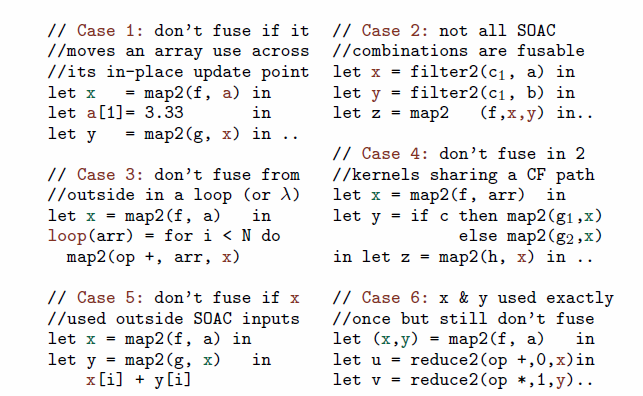
\includegraphics[width=0.6\textwidth]{images/cases.png}
  \caption{Don't Fuse Cases \cite[page 6]{T2Fusion}}
  \label{fig:cases}
\end{figure}

\begin{itemize}
\item[Case 1:] Fusion across a in-place update is not possible. When fusing the producer array is not created as before, but a part of the computation in the resulting fused SOAC.
\item[Case 2:] Not all combinations of SOACs are fusable.
\item[Case 3:] Fusion across a loop or a SOAC lambda would duplicate the computation and potentially change the time complexity of the program. In this case instead of calculating variable x once, a fusion would result in x being calculated in each of the loops. 
\item[Case 4:] When the array x produced by a SOAC is consumed by two other SOACs located on the same execution path, the computation will be duplicated.
\item[Case 5:] If array x produced by SOAC is used other then input to another SOAC fusion is not allowed.
\item[Case 6:] If two arrays created by a SOAC is used as input in more then one SOAC the computaion is duplicated, and fusion is therefore not allowed.
\end{itemize}

However there are special cases for scanomap, as the result array x of the producer SOAC in the scanomap transformation, also will be returned by the scanomap in cases where other SOACs consumes array x.


\subsection{Fusing Scanomap}
% What can we not reduce with
Once a \texttt{map} and a \texttt{scan} has been combined into a \texttt{scanomap}, it raises the question of how can we further fuse this new construct?
 This section details which SOACs \texttt{scanomap} can fuse with, and how.
\paragraph{Map-Scanomap Fusion}
Fusing a \texttt{map} as a producer into a consumer \texttt{scanomap} is a simple process. Given a \texttt{map} with function $g$ and a 
 \texttt{scanomap} with the folding function $\odot_f$, we compose a new folding function $x \odot_{f \circ g} y = x \odot f (g (y))$. This is illustrated below,
\begin{align*}
  b &= \mathtt{map} \: g \: a \\
  c &= \mathtt{scanomap} \: \odot \: \odot_f \: e \: b \\
\Downarrow \\
  c &= \mathtt{scanomap} \: \odot \: \odot_{f\circ g} \: e \: a\mathnormal{.}
\end{align*}

\paragraph{Scanomap-Scanomap Fusion} Horizontally fusing a \texttt{scanomap} with another \texttt{scanomap}, requires that theres exists no dependency between the
 two SOACs -- i.e. there exists no producer-consumer relationship between the two. In theses cases, it may still prove beneficial to perform fusion -- even though there is no direct
 optimisation -- to enable more fusion.
% Tuples
This kind of fusion is performed by in a way concatenating input, output, and both functions for the input \texttt{scanomaps}, which gives the following,
\begin{align*}
  c &= \mathtt{scanomap} \: \odot_1 \: {\odot_1}_f \: e_1 \: a \\
  d &= \mathtt{scanomap} \: \odot_2 \: {\odot_2}_g \: e_2 \: b \\
\Downarrow \\
  (c,d) &= \mathtt{scanomap} \: \odot' \: \odot'_{fg} \: (e_1, e_2) \: (a, b)\mathnormal{.}
\end{align*}
Where $\odot'(e_1,e_2, x, y) = (e_1 \odot x, e_2 \odot y)$ and $\odot'_{fg}(e_1, e_2, x, y) = (e_1 \odot f(x), e_2 \odot f(y))$. In this way, the resulting \texttt{scanomap}
 now describes the computations of both input \texttt{scanomap}s.
\section{Implementation}
% How does a futhark program look ~ absyn. As we need it.
This section will detail the specifics of performing \texttt{map-scan}, and other \texttt{scanomap} fusions, as well as detailing the process of
 analysing a program for valid fusions.

\subsection{Program State}
There are a series of conditions for the fusion transformation can happen. As well as a number of cases where a fusion should not happen. The fusion transformation assumes a normalized program, with the following properties: \cite[Figure 5, page 4]{T2Fusion} 

\begin{itemize}
\item No tuple type can appear in an array or tuple type, i.e., flat
tuples,
\item unzip has been eliminated, zip has been replaced with assertZip,
which verifies either statically or at runtime that the outer size of zip’s input matches, and finally, the original SOACs (map)
have been replaced with their tuple-of-array version,
\item tuple expressions can appear only as the final result of a function,
SOAC, or if expression, and similarly for the tuple pattern
of a let binding, e.g., a formal argument cannot be a tuple,
\item $\: e_1$ cannot be a let expression when used in let $\: p$ = $\: e_1$ in $\: e_2$,
\item each if is bound to a corresponding let expression, and
an if’s condition cannot be in itself an if expression, e.g., \\
$\: a$ + if( if $\: c_1$ then $\: e_1$ else $\: e_2$ ) then $\: e_3$ else $\: e_4$ $\rightarrow$ \\
let $\: c_2$ = if $\: c_1$ then $\: e_1$ else $\: e_2$ in \\
let $\: b$ = if $\: c_2$ then $\: e_3$ else $\: e_4$ in $\: a+ \:b$ 
\item function calls, including SOACs, have their own let binding, e.g., \\
reduce2($\:f,\:a$) + $\:x$ $\Rightarrow$ let $\:y$ = reduce2($\:f,\:e,\:a$) in $\:y+\:x$,
\item all actual arguments are vars, e.g., $\:f(\:a+\:b))$ $\Rightarrow$ let $\:x=\:a+\:b$ in $\:f(\:x)$.
\end{itemize}
The properties listed above is reached by going through the different stages in the compiler pipeline, as shown in figure \ref{fig:pipeline}. Type checking first so that any errors will refer to the actual names given by the programmer, then moving on to tuple transformation that flattens all tuples and converts arrays of tuples to tuples of arrays. Tuple and let normalisation to optimise the code based on code recognition (e.g $\:f(\:a+\:b)) \Rightarrow$ let $\:x=\:a+\:b$ in $\:f(\:x)$).

\begin{figure}[hb!]
  \centering
    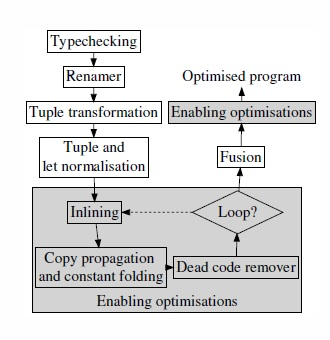
\includegraphics[width=0.5\textwidth]{images/pipeline.jpg}
  \caption{Compile pipeline \cite[page 4]{T2Fusion}}
  \label{fig:pipeline}
\end{figure}

When the program has reached the properties mentioned it enters the enabling optimisations loop, with aggressive in lining (i.e., building the call-graph and moving non recursive functions into the function calling it.). Copy propagation e.g., 
$$y = x $$
$$z = 5 * y $$
Would become
$$z = 5 * x $$
and constant folding where the compiler evaluating constant expressions at compile time. After dead code removal the process repeats unless a fixed point is reached, if the fixed point is reached the program is ready for possible fusion transformations.

\subsection{Bottom Up Analysis}
% How the fusion module analyses the program
Futhark's fusion module gathers fusible SOACs by using a bottom-up analysis pass of the program's AST. This is done by traversing the AST depth first, while using a set
 of environments and data structures, to among other things keep track created kernels and the production and consumption of arrays. \cite{T2Fusion}

These are structures and environments are filled out during the depth first traversal of the AST, such that when analysing a specfic SOAC in the program it is known which
 SOACs consume its outputs, and whether in-place update in between and so on.

For example, when analysing the program found in Figure \ref{fig:progsnip1} and the looking at the \texttt{map} statement, two simple look-ups will show that while $b$ is consumed by the
 \texttt{scan}, it is consumed by an in-place updated previously. Hence, fusion is not possible.
\begin{figure}[hb!]
  \centering
  \begin{mdframed}[style=alignbox]
  \begin{align*}
    &\phantom{---}\vdots\\
    &\lett b = \mathtt{map} \: f \: a \inn\\
    &\lett b[1] = 4 \inn\\
    &\lett c = \mathtt{scan} \: \odot \: 0 \: b \inn\\
    &\phantom{---}\vdots
  \end{align*}
\end{mdframed}

  \caption{Infusible program snippet.}
  \label{fig:progsnip1}
\end{figure}

Fusion is then attempted along the way whenever the fusion module meets a new SOACs during its analysis. Consequently, we have that fusion is also performed bottom-up, such that
 the compiler will prioritize potential fusion by how ``deep'' the candidates occur in the program.
\subsection{Map-Scanomap Fusion}
\setcounter{equation}{0}
Having identified a single \texttt{map} producer and a \texttt{scanomap} consumer to perform fusion on, the fusion itself may seem fairly simple.
 However, this is not entirely the case in most situations, as especially function composition isn't as straight forward as it can seem. There are also two factors
 which complicate this process:
 \begin{itemize}
 \item As previously mentioned, all SOACs in Futhark work with tuples of arrays. This means that a $b = \mathtt{map}\: f \: a$ is actually short hand for
$(b0, b1, .. ,bn) = \mathtt{map} \: f \: (a0, a1, ..., an)$, and not all members of the same tuples are consumed, or produced, in the same place.
 \item Certain SOACs in Futhark support map-out arrays -- i.e. array-outputs from a fused \texttt{map} which are still output after fusion. This is also
 supported by \texttt{scanomap}. 
 \end{itemize}
This section will go through the algorithm for fusing a single \texttt{map} into a \texttt{scanomap} -- and by extension the algorithm for fusing a \texttt{map} into a \texttt{scan}.

The function inputs of SOACs in Futhark consist of a set of parameters, a set of \texttt{let} bindings, and a body which defines the function output. When
 looking to create a new folding function for the resulting \texttt{scanomap} construct, composed entirely from the functions found in the to-be-fused \texttt{map} and \texttt{scanomap}.
\begin{figure}[h!]
  \centering
  \begin{align}
    &f (a0, a1, a2, a3) = \\
    &\lett (x1,x2) = g(a0, a1) \inn \\
    &\lett y1 = a2 + a3 \inn \\
    &(x1, x2, y1)
  \end{align}
  \caption{Example of a SOAC lambda function.}
\end{figure}
Firstly, we will find the new parameter set for the new folding function. Given a program, wherein a \texttt{map} is to be fused with a \texttt{scanomap} into a new \texttt{scanomap}:
\begin{align*}
b &= \mathtt{map} \: f \: a \\
d &= \mathtt{scanomap} \: \odot \: \odot_g \: ne \: c \mathnormal{.}  
\end{align*}
Where $a, b, c, d$ are all tuples of arrays, and $ne$ is a tuple of neutral elements.

Fusing these two SOACs into a \texttt{scanomap} becomes a three step process of
\begin{enumerate}
\item determining the parameter list of the output \texttt{scanomap},
\item determining map-out arrays, and
\item composing a new folding function.
\end{enumerate}
Afterwards a new \texttt{scanomap} can then be constructed which can replace the input \texttt{map} and \texttt{scanomap}.
\paragraph{Parameters}

We have that \texttt{map} and \texttt{scanomap} are to be fused, so we must also have $(b0, b1, ...,bn) \cap (c0, c1, ..., cn) \neq \emptyset$. However
 we do not neccessarily have $(b0, b1, ...,bn) = (c0, c1, ..., cn)$. The parameters for our fused product must then become all of the array input parameters from the \texttt{map} as well as
 the array input parameters from the \texttt{scanomap} which aren't produced by the \texttt{map}. Hence, our new list of parameters become,
$$\text{New-Params} = (a \cup c) / b\mathnormal{.}$$


\paragraph{Map-Out Arrays}
Next is to find any map-out arrays which need to be returned. These can potentially consist of some subset of the output arrays of both the \texttt{map} and the \texttt{scanomap}. The map-out arrays
 already carried by the input \texttt{scanomap} are by convention placed last in the list of outputs, so they correspond to the $\mathtt{len}(d) - \mathtt{len}(ne)$ last members of $d$.
$$\text{map-out}_{scanomap} = \mathtt{drop}(\mathtt{len}(ne),d)$$

The map-out arrays from the input \texttt{map} are found by using the fusion environment
 -- which keeps track of where arrays are consumed -- through the \texttt{unfus} function which
 filters out any arrays which are not consumed later in the program.
$$\text{map-out}_{map} = \mathtt{unfus} (b)$$

Combining these two tuples will then give us the full set of map-out arrays for the fused product,
$$\text{map-out} = m_{out} = \mathtt{drop}(\mathtt{len}(ne),d) \doubleplus \mathtt{unfus} (b)\mathnormal{.}$$
\paragraph{Function Composition}
\setcounter{equation}{0}
Composing the folding function for the resulting \texttt{scanomap} from the input \texttt{map}'s $f$ function, and the input \texttt{scanomap}'s $\odot_g$ function is a question of combining their
 bindings such that the result of the $f$ function is computed first and bound such that it can be used to compute $\odot_g$.

The input functions will both consist of some amount of let bindings followed by a body which consists solely of the variables to be returned. Figure \ref{fig:bothfuns} shows generalized functions for both
 inputs where $a_i$ is the tuple consisting of the $i$th elements of the arrays contained in the $a$ tuple. 
 \begin{figure}[hb!]

   \begin{mdframed}
 \begin{minipage}{0.5\linewidth}
     \centering

       \begin{align*}
         &f(a_i) = \\
         &\lett x_1 = e_1 \inn\\
         &\lett x_2 = e_2 \inn\\
         &\phantom{----}\vdots\\
         &\lett x_n = e_n \inn\\
         &b_i
       \end{align*}

     \label{fig:mapf}
 \end{minipage}
 \begin{minipage}{0.5\linewidth}
     \centering

     \begin{align*}
       &\odot_f(ne, c_i) = \\
       &\lett y_1 = e_1 \inn\\
       &\lett y_2 = e_2 \inn\\
       &\phantom{----}\vdots\\
       &\lett y_n = e_n \inn\\
       &d_i
     \end{align*}

     \label{fig:odotg}
   \end{minipage}

     \end{mdframed}
     \caption{The SOAC functions $f$ and $\odot_g$ from the input
       \texttt{map} and \texttt{scanomap}.}
     \label{fig:bothfuns}
\end{figure}

Combining these two functions into a single new folding function $\odot_g \circ f$ (or $\odot_{g \circ f}$) is then a question of first applying all of the bindings
 from the $f$ function, creating a new binding which binds the body of $f$ to the corresponding parameters of $\odot_g$, and then on
 to that appending the bindings of $\odot_g$.


\begin{figure}[h!]\centering
  \begin{mdframed}[style=alignbox]
    \begin{align*}
      &\odot_{g} \circ f(ne, ((a \cup c) / b)_i) = \\
      &\lett x_1 = e_1 \inn\\
      &\lett x_2 = e_2 \inn\\
      &\phantom{----}\vdots\\
      &\lett x_n = e_n \inn\\
      &\lett c_i = b_i \inn\\
      &\lett y_1 = e_1 \inn\\
      &\lett y_2 = e_2 \inn\\
      &\phantom{----}\vdots\\
      &\lett y_n = e_n \inn\\
      &(d_i /m_{out_i}) \doubleplus m_{out_i}
    \end{align*}
  \end{mdframed}

  \caption{Resulting function $\odot_{f \circ g}$.}
  \label{fig:fusresfun}
\end{figure}
The body of $\odot_{f\circ g}$ then becomes the outputs of $\odot_g$ minus any map-out arrays appended with the new map-out arrays as
 found above.

We can then replace the original \texttt{map} and \texttt{scanomap} with a new \texttt{scanomap},
$$(d / m_{out}) \doubleplus m_{out} = \mathtt{scanomap} \: \odot \: \odot_{f \circ g} \: ne \: \left((a \cup c) / b \right)\mathnormal{.} $$
% Detail map and scanomap constructions incl. functions, order of parameter arrays, and map-out arrays
% Go through how we disassemble their functions, and reassemble a new function:
% - 
% How is the new Scanomap construct formed.

\subsection{Scanomap-Scanomap Fusion}
Having two \texttt{scanomap} in a futhark program with no dependencies between the two SOACs, and equal length input, the program computation time can be optimised using horizontal fusion. 

This section will go through the algorithm for fusing two \texttt{scanomap} into one \texttt{scanomap}. The fusion algorithm have two steps:
\begin{enumerate}
\item Composing a new assosiative operation
\item Composing a new folding function.
\end{enumerate}

\begin{align*}
  c &= \mathtt{scanomap} \: \odot_1 \: {\odot_1}_f \: e_1 \: a \\
  d &= \mathtt{scanomap} \: \odot_2 \: {\odot_2}_g \: e_2 \: b \\
\Downarrow \\
  (c,d) &= \mathtt{scanomap} \: \odot' \: \odot'_{fg} \: (e_1, e_2) \: (a, b)\mathnormal{.}
\end{align*}


\paragraph{Parameters} With two \texttt{scanomap} to be fused, the goal is to join the computations within the same loop. Hence $\: a$ does not have to equal $\: b$, but the the length of the input arrays must be the same. Our new list of parameters simply become:
$$\text{New-Params} = (a,b)$$

\paragraph{New folding function and associative operation} As the two \texttt{scanomap} are independent of each other the composition of the new fused folding function is fairly easy. Figure \ref{fig:pre-fusion} show the pre-fusion folding functions for both scanomap, running sequentially after each other. Fusing them is simply adding the additional parameters and adding the function body of one of them into the other as shown in figure \ref{fig:post-fusion}. 

\clearpage
 \begin{figure}[hb!]

   \begin{mdframed}
 \begin{minipage}{0.5\linewidth}
     \centering

       \begin{align*}
       &\odot_f(ne_1, a_i) = \\
       &\lett x_1 = e_1 \inn\\
       &\lett x_2 = e_2 \inn\\
       &\phantom{----}\vdots\\
       &\lett x_n = e_n \inn\\
       &c_i
       \end{align*}

     \label{fig:mapf}
 \end{minipage}
 \begin{minipage}{0.5\linewidth}
     \centering

     \begin{align*}
       &\odot_g(ne_2, b_i) = \\
       &\lett y_1 = e_1 \inn\\
       &\lett y_2 = e_2 \inn\\
       &\phantom{----}\vdots\\
       &\lett y_n = e_n \inn\\
       &d_i
     \end{align*}

     \label{fig:odotg}
   \end{minipage}

     \end{mdframed}
     \caption{The SOAC functions $\odot_f$ and $\odot_g$ from the two scanomap}
     \label{fig:pre-fusion}
\end{figure}

\begin{figure}[hb!]

   \begin{mdframed}
     \centering

       \begin{align*}
       &\odot'_{fg}(ne1, ne2, a_i, b_i ) = \\
       &\lett x_1 = e_1 \inn\\
       &\lett x_2 = e_2 \inn\\
       &\phantom{----}\vdots\\
       &\lett x_n = e_n \inn\\
       &\lett y_1 = e_1 \inn\\
       &\lett y_2 = e_2 \inn\\
       &\phantom{----}\vdots\\
       &\lett y_n = e_n \inn\\
       &(c_i, d_i)
       \end{align*}
       \end{mdframed}
     \caption{Fused function $\odot'_{fg}$}
     \label{fig:post-fusion}
\end{figure}

In the same manor the assosiative operations is fused into one, enabling the computation of two scanomaps to be done within one loop. 

\paragraph{Map-Out Arrays}
If the map-out arrays in the \texttt{scanomaps} should be returned, it is done in the same manor as explained in the consumer-producer fusion of map and scan in section Map-Scanomap Fusion. Because the horizontally fused \texttt{scanomaps} are computed in precisely the same way, just "sequentially" in one loop it does not change anything regarding map-out arrays.

% Conditions
% Function composition
\subsection{Other Fusion}




% Algoritmical description of of the fusion process: function composition, determining input/outputs of fusion products.
% Detailed descriptions of relevant parts.

\section{Benchmarking and Testing}
%How have we tested our implementation. Does it work? Why?\\
%How does the performance of a fused program compare with a non-fused program both %sequentially and parallelly. Why?

In this section we will go through how we have tested our implementation, and the benchmark results. 

\subsection{Tests}

Testing the computation time improvement is done with this simple Futhark program. 

\begin{lstlisting}[caption=Test program] 
fun ([int]) main([int] inp) =
  let a = map(+10, inp)
  let b = scan(+, 0, a) in
  (b)
\end{lstlisting}

The test program contains a simple map producer and scan consumer, with the scanomap implementation the resulting program will be one scanomap. By testing with and without the scanomap implementation, the results will show us any increase/decrease in computation time. We run the test program with increasingly large amount of data, and several times per data amount to try and negate any large deviations.

\subsection{Benchmarks}

\section{Conclusion}
\newpage

\bibliographystyle{unsrt}
\bibliography{lit}

\end{document}